\documentclass[a5paper]{article}

\usepackage{amsmath, amssymb}
\usepackage{multicol}
\setlength{\columnsep}{1cm}
\usepackage[margin=0.75in]{geometry}
\usepackage{graphicx}
\graphicspath{ {../../../Images/ENEE12015/} }
\usepackage[breaklinks, hidelinks]{hyperref}
\usepackage{siunitx}
\usepackage{tikz}
\usetikzlibrary{patterns, positioning, arrows.meta, matrix, fit, calc}
\usepackage{xcolor}
\usepackage[american]{circuitikz}
\usepackage{pgfplots}
\pgfplotsset{compat=newest}
\usepgfplotslibrary{external}
\usepackage{stix}
\usepackage{ragged2e}
\usepackage{enumitem}
\usepackage{polynom}

\newcommand{\minus}{\scalebox{0.5}[1.0]{$-$}}
\newcommand{\sech}{\mathrm{sech}}
\newcommand{\csch}{\mathrm{csch}}
\newcommand{\Lap}{\mathcal{L}}
\newcommand{\For}{\mathcal{F}}
\setcounter{secnumdepth}{4}
\renewcommand\paragraph{\@startsection{paragraph}{4}{\z@}%
% display heading, like subsubsection
                                     {-3.25ex\@plus -1ex \@minus -.2ex}%
                                     {1.5ex \@plus .2ex}%
                                     {\normalfont\normalsize\bfseries}}
\sisetup{
	round-mode = places,
	round-precision = 2,
}

\date{5\textsuperscript{th} of November 2026}

\begin{document}
	\begin{titlepage}
		\centering
		{\Huge \textsc{ENEE12015 - Electrical Power Engineering}\par}
		\vspace{1cm}
		{\Large \textsc{Lecture Notes}\par}
		\vspace{2.5cm}
		\vfill
		Authored by\par
		Lachlan J. W. Wyer
		\vfill
		\makeatletter
		{\large Document Start Date: \@date \par}
		\makeatother
		{\large Latest Update: \today\par}
	\end{titlepage}
	\tableofcontents
	\pagebreak
	
	\section{Introduction to Electrical Power Systems}
	\subsection{Early Development:}
	1800's - Electricity and Magnetism well understood intellectually\\
	1831 - Magnetica field was discovered to generate electricity\\
	1845 - First commerical operations of telegraph\\
	1860 - First electrical generator\\
	1870 - First incandesent light bulb\\
	1882 - First commericial power system in NY City\\
	1883 - Polyphase induction motor\\
	1885 - Commericial availability of AC power

	\subsection{Power System Compenets:}
	\begin{itemize}
		\item Generators
		\item Transformers
		\item Transmission lines
		\item Substations/Terminal Stations
		\item Distribution lines
		\item Electrical loads
	\end{itemize}
	When transmitting power, the best senario is high voltage, low current transmission. Ideally below the resistivity of the power lines.

	\subsection{Power System Models:}
	\subsubsection{Generators}
	\begin{center}
	\begin{circuitikz}[line width=0.8pt]
	  % AC Voltage Source
	  \draw (0,0) to[sV, l=$E_g$] (0,3)
		-- (1.0,3);

	  % Resistor and Inductor inside Impedance Box
	  \draw (1.0,3) to[R] (2.6,3) 
		to[L] (4.2,3)
		to[short, -o] (5.0,3);

	  % Enclosing Box for Impedance Z_g
	  \draw[line width=0.6pt] (0.8,2.3) rectangle (4.4,3.5);
	  \node at (2.6,1.8) {\large $Z_g$};

	  % Bottom wire and terminal node
	  \draw (0,0) -- (5.0,0) node[circ, open] {};

	  % Output Current Arrow
	  \draw[->, >=stealth, line width=0.8pt] (4.9,3.4) -- (5.5,3.4) node[right] {\large $I_g$};

	  % Output Voltage Polarity and Label
	  \node at (5.0,2.4) {\large $+$};
	  \node at (5.0,1.5) {\large $V_g$};
	  \node at (5.0,0.6) {\large $-$};
	\end{circuitikz}
	\end{center}
	\subsubsection{Transmission/Distribution Lines}
	\begin{center}
	\begin{circuitikz}[line width=0.8pt]
	  % Left terminal vertical bars
	  \draw (0, 2.7) -- (0, 3.3);
	  \draw (0, -0.3) -- (0, 0.3);

	  % Top-left wire & Current arrow
	  \draw (0,3) -- (2,3) node[circ] {};
	  \draw[->, >=stealth, line width=0.8pt] (0.6, 3.4) -- (1.4, 3.4) node[midway, above] {$I_{Z_g}$};

	  % Left Voltage V_g
	  \node at (0.5, 2.2) {$+$};
	  \node at (0.5, 1.5) {\large $V_g$};
	  \node at (0.5, 0.8) {$-$};

	  % Left shunt capacitor
	  \draw (2,3) to[C] (2,0) node[circ] {};
	  \node[right] at (2.1, 1.5) {\large $-j 2 X_c$};

	  % Series branch: Resistor + Inductor in Impedance Box
	  \draw (2,3) -- (2.8,3);
	  \draw (2.8,3) to[R] (4.4,3) to[L] (6.0,3);
	  \draw (6.0,3) -- (6.8,3) node[circ] {};

	  % Rectangle box for Z = R + jX_L
	  \draw[line width=0.6pt] (2.6, 2.3) rectangle (6.2, 3.5);
	  \node at (4.4, 1.8) {\large $R + j X_L$};

	  % Right shunt capacitor
	  \draw (6.8,3) to[C] (6.8,0) node[circ] {};
	  \node[left] at (6.7, 1.5) {\large $-j 2 X_c$};

	  % Top-right wire
	  \draw (6.8,3) -- (8.8,3);

	  % Bottom wire & Ground
	  \draw (0,0) -- (8.8,0);
	  \draw (4.4,0) node[circ] {} node[ground] {};

	  % Right terminal vertical bars
	  \draw (8.8, 2.7) -- (8.8, 3.3);
	  \draw (8.8, -0.3) -- (8.8, 0.3);

	  % Right Voltage V_q
	  \node at (8.3, 2.2) {$+$};
	  \node at (8.3, 1.5) {\large $V_q$};
	  \node at (8.3, 0.8) {$-$};
	\end{circuitikz}
	\end{center}
	\subsubsection{Transformers}
	\begin{center}
	\begin{circuitikz}[scale=0.75, transform shape, line width=0.7pt]

	    % Left Port Terminals & Voltage Vg
	    \coordinate (in_top) at (0, 4);
	    \coordinate (in_bot) at (0, 0);
	    \draw (in_top) node[ocirc]{};
	    \draw (in_bot) node[ocirc]{};
	    \node at (0, 3.2) {$+$};
	    \node at (-0.4, 2) {\Large $V_g$};
	    \node at (0, 0.8) {$-$};

	    % Right Port Terminals & Voltage VT
	    \coordinate (out_top) at (10, 4);
	    \coordinate (out_bot) at (10, 0);
	    \draw (out_top) node[ocirc]{};
	    \draw (out_bot) node[ocirc]{};
	    \node at (10, 3.2) {$+$};
	    \node at (10.4, 2) {\Large $V_T$};
	    \node at (10, 0.8) {$-$};

	    % Z1 Branch (Resistor + Inductor in series inside a box)
	    \coordinate (z1_in)  at (1, 4);
	    \coordinate (z1_out) at (4.2, 4);
	    \draw (in_top) -- (z1_in);
	    \draw (z1_in) to[R, name=R1] (2.6, 4) to[L, name=L1] (z1_out);
	    \node[draw, rectangle, inner sep=6pt, fit={(R1) (L1)}, label=below:$Z_1$] {};

	    % Central Top Node & Current Im
	    \coordinate (node_top) at (5, 4);
	    \coordinate (par_top)  at (5, 3.1);
	    \draw (z1_out) -- (node_top) node[circ]{};
	    \draw[->, >=stealth, thick] (node_top) -- (par_top) node[midway, left] {$I_m$};

	    % Z2 Branch (Resistor + Inductor in series inside a box)
	    \coordinate (z2_in)  at (5.8, 4);
	    \coordinate (z2_out) at (9, 4);
	    \draw (node_top) -- (z2_in);
	    \draw (z2_in) to[R, name=R2] (7.4, 4) to[L, name=L2] (z2_out);
	    \node[draw, rectangle, inner sep=6pt, fit={(R2) (L2)}, label=below:$Z_2$] {};
	    \draw (z2_out) -- (out_top);

	    % Magnetizing Parallel Branch (Rm || jXm)
	    \coordinate (par_bot) at (5, 0.9);
	    \draw (par_top) node[circ]{} -- (3.8, 3.1) to[R, l_=$R_m$] (3.8, 0.9) -- (par_bot);
	    \draw (par_top) -- (6.2, 3.1) to[L, l=$jX_m$] (6.2, 0.9) -- (par_bot) node[circ]{};

	    % Bottom Wire and Ground Connection
	    \coordinate (node_bot) at (5, 0);
	    \draw (par_bot) -- (node_bot) node[circ]{};
	    \draw (in_bot) -- (out_bot);

	\end{circuitikz}
	\end{center}
	\subsubsection{Loads}
	\begin{center}
	\begin{circuitikz}[scale=0.75, transform shape, line width=0.7pt]
	    % Left Port Terminals & Voltage Vg
	    \coordinate (in_top) at (0, 3.5);
	    
	    \draw (in_top) node[ocirc]{};
	    \draw (0, 0) node[ground]{};
	    
	    % Voltage polarity and label
	    \node at (0, 2.7) {$+$};
	    \node at (-0.4, 1.75) {\Large $V_g$};
	    \node at (0, 0.8) {$-$};

	    % Top Wire with Current Arrow IL ->
	    \coordinate (load_top) at (4, 3.5);
	    \draw (in_top) -- (load_top) node[midway, above=2pt] {$I_L \longrightarrow$};

	    % Z_load Branch (Resistor + Inductor in series inside box)
	    \coordinate (load_bot) at (4, 0);
	    \draw (load_top) to[R, name=Rload] (4, 2.0) to[L, name=Lload] (4, 0.5) -- (load_bot) node[ground]{};

	    % Bounding Box labeled Z_load
	    \node[draw, rectangle, inner xsep=8pt, inner ysep=10pt, fit={(Rload) (Lload)}, label=right:\Large $Z_{\text{load}}$] {};

	\end{circuitikz}
	\end{center}

	\subsection{Basic Theory:}
	Ohm's Law - $V=IZ$\\
	KVL - $\sum V=0$\\
	KCL - $\sum I_{in}=\sum I_{out}$\\
	Power Flow - $S=P+jQ=VI^{*}$
	\subsection{Current and Power Flow:}
	\begin{itemize}
		\item Technically current flow within an AC system is arbitrary
		\item Power is clear from source to load
		\item Steady state is only assumed
	\end{itemize}
	\subsection{Power in AC Circuits:}
	Average Power over time period T
	$$P=\frac{1}{T}\int^{t_{0}+T}_{t_{0}}v(t)i(t)dt$$
	Instantaneous Power
	$$p(t)=v(t)i(t)$$
	When a circuit is in steady state, all voltages and currents become sinusodial. The periodic nature of the waveforms enables more specific derivation of power relationships.
	$$P_{av}=\frac{E_{m}I_{m}}{2}=\frac{E_{m}}{\sqrt{2}}\times\frac{I_{m}}{\sqrt{2}}=E_{RMS}I_{RMS}$$
	This only works when $v(t)$ and $i(t)$ are in phase. When a small phase shift occurs:
	$$P_{av}=\frac{E_{m}I_{m}}{2}\cos{(\theta)}=E_{RMS}I_{RMS}\cos{(\theta)}$$
	When $i(t)$ lags $v(t)$ by $90^{\circ}$
	$$P_{av}=E_{RMS}I_{RMS}\cos{(90^{\circ})}=0$$
	\subsection{Reactive Power:}
	Power that dose no useful work within a system.
	$$Q=E_{RMS}I_{RMS}\sin{(\phi))}$$
	VAR is a defined value and does not relate to the area under P. When $v(t0$ and $i(t)$ are in phase ($\phi=0$), $Q=0$. When reactive power is maximum ($\phi=90^{\circ}$), $Q=E_{RMS}I_{RMS}$ and $P_{av}=0$.
	
	\subsection{Power Triangles:}
	\begin{center}
	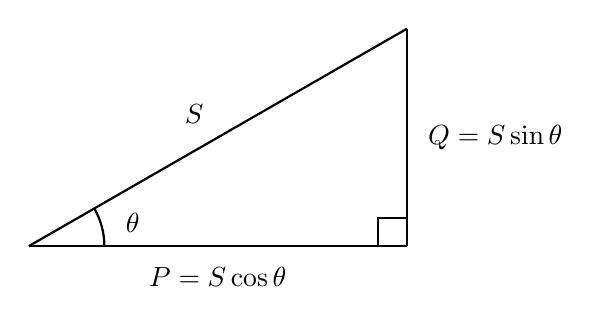
\begin{tikzpicture}[scale=1.2, line width=0.8pt]
	    % Coordinates
	    \coordinate (A) at (0, 0);
	    \coordinate (B) at (4, 0);
	    \coordinate (C) at (4, 2.3);

	    % Right angle symbol
	    \draw (3.7, 0) -- (3.7, 0.3) -- (4, 0.3);

	    % Triangle edges and side labels
	    \draw (A) -- (B) node[midway, below=4pt] {$P = S \cos\theta$};
	    \draw (B) -- (C) node[midway, right=4pt] {$Q = S \sin\theta$};
	    \draw (C) -- (A) node[midway, above left=2pt] {$S$};

	    % Angle theta arc and label
	    \draw (0.8, 0) arc (0:29.9:0.8);
	    \node at (1.1, 0.25) {$\theta$};

	\end{tikzpicture}
	\end{center}
	Q is wished to be minised, allowing the maximum S to used within the load (active power) usefully.

	\subsection{Power Flow Direction:}
	A positive P present in a power triangle indicates that $\phi$ is between $-90^{\circ}$ and $90^{\circ}$. With a negative P show $\phi$ to be $>90^{\circ}$. It is necessary to assign a current direction in AC circuits, for the purpose of writing equations in a consistent manner. $Q>0$, flowing in the same direction as current is assumed to go. $Q<0$, flowing apposed to the assumed current direction.\\
	Power Factor:
	$$pf=\frac{P}{S}=\cos(\phi)$$

	\section{Three Phase Power}
	\subsection{What is it?:}
	A 3-phase power system is just a connecting of 3 singlephase systems together for set operation. Each phase must operate at the same voltage and current magnitudes seperated by $120^{\circ}$ phase angle.
	\subsection{Balanced Operating Conditions:}
	Under normal operating conditions all voltages, current, $120^{\circ}$ angle shift and loads contain same characteristics.
	\subsection{Analysis of 3-Phase:}
	Assuming a system is under balanced conditions, means that only a single phase system needs to be analysed. Faults, abnormal load conditions, cause a system to become unbalanced.
	\subsection{Popularity of Polyphase Systems:}
	Polyphase machines can be designed to operate under constant total power conditions. Hence, these machines have smoother operations. These machines are then simpler to design, how all as tansmission lines can delivers greater power for less cost.
	\subsection{Power in Polyphase Systems:}
	Single Phase: Resistive
	\begin{center}
	\begin{circuitikz}[scale=0.75, transform shape, line width=0.7pt]
	    % ================= LEFT DIAGRAM: ARMATURE CIRCUIT ================= Stator / Armature Circle
	    \draw[thick] (0, 1.8) circle (1.0);
	    
	    % Internal terminals & coil markings
	    \draw (0.3, 2.3) node[ocirc]{} node[right=1pt, font=\small] {$a$};
	    \draw (-0.3, 2.3) node[ocirc]{} node[left=1pt, font=\small] {$b$};
	    \draw (-0.3, 1.3) node[ocirc]{} node[left=1pt, font=\small] {$a'$};
	    \draw (0.3, 1.3) node[ocirc]{} node[right=1pt, font=\small] {$b'$};

	    % Internal curved arrows (rotation / winding direction)
	    \draw[->, >=stealth, thin] (0.2, 2.0) arc (30:-30:0.4);
	    \draw[->, >=stealth, thin] (-0.2, 1.6) arc (210:150:0.4);

	    % Top wire with current ia arrow
	    \draw (0.3, 2.3) -- (0.3, 3.2) -- (3.2, 3.2) node[midway, above] {$i_a \longrightarrow$};
	    
	    % Bottom return wire from a'
	    \draw (-0.3, 1.3) -- (-0.3, 0.4) -- (3.2, 0.4);

	    % Load Box containing Resistor
	    \draw (3.2, 3.2) -- (3.2, 2.5) to[R, name=Rload] (3.2, 1.1) -- (3.2, 0.4);
	    \node[draw, rectangle, inner xsep=8pt, inner ysep=6pt, fit={(Rload)}] {};

	    % Induced Voltage Polarity & Label
	    \node at (3.8, 2.4) {$+$};
	    \node at (4.0, 1.8) {\Large $e_a$};
	    \node at (3.8, 1.2) {$-$};


	    % ================= RIGHT DIAGRAM: EMF WAVEFORMS =================
	    \begin{scope}[shift={(6.0, 1.8)}]
		% Horizontal and Vertical Axes
		\draw[->, >=stealth, thick] (0, 0) -- (4.2, 0);
		\draw[<->, >=stealth, thick] (0, -2.2) -- (0, 2.5);

		% Multi-coil Induced EMF Pulsating Waveforms
		% Envelope / Main rectified wave
		\draw[thick, smooth, domain=0:3.8, samples=100] 
		    plot (\x, {1.5*abs(cos(deg(\x*1.3)))});

		% Phase-shifted coil component 1
		\draw[thick, smooth, domain=0:3.8, samples=100] 
		    plot (\x, {1.2*sin(deg(\x*1.5 + 0.8))});

		% Phase-shifted coil component 2
		\draw[thick, smooth, domain=0:3.8, samples=100] 
		    plot (\x, {0.8*cos(deg(\x*1.1 - 0.2))});
	    \end{scope}

	\end{circuitikz}
	\end{center}
	\begin{align*}
		p_{a}=&e_{a}i_{a}\\
		=&E_{m}I_{m}\cos^{2}(\omega t)\\
		P_{av}=&E_{RMS}I_{RMS}\\
	\end{align*}
	2-Phase: Resistive
	\begin{center}
		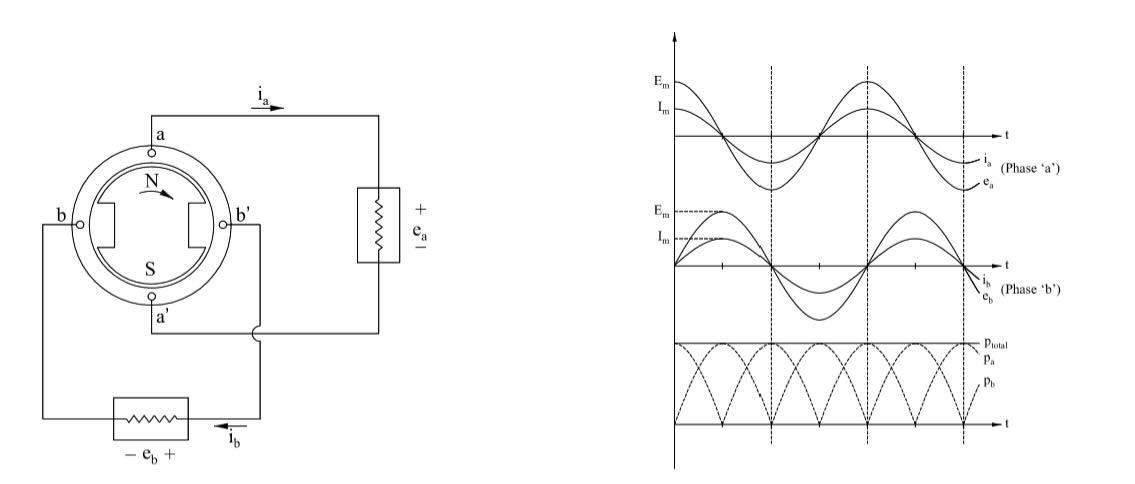
\includegraphics[scale=0.25]{2-phase-resistive.png}
	\end{center}
	Voltage induced in b-b' lags voltage in a-a' by 90 electrical degrees. In 2-pole machines, 1 electrical degree is equivalent to 1 mechanical degree.
	\begin{align*}
		e_{a}&=E_{m}\cos(\omega t)\\
		i_{a}&=I_{m}\cos(\omega t)\\\\
		e_{b}&=E_{m}\cos(\omega t-90^{\circ})\\
		&=E_{m}\sin(\omega t)\\
		i_{b}&=I_{m}\cos(\omega t-90^{\circ})\\
		&=I_{m}\sin(\omega t)\\\\
		P_{Tot}&=P_{a}+P_{b}\\
		&=E_{m}I_{m}\cos^{2}(\omega t)+E_{m}I_{m}\sin^{2}(\omega t)\\
		&=E_{m}I_{m}
	\end{align*}
	There are two seperate loads. This $P_{Tot}$ is true as long as the load is the same.
	\begin{align*}
		P_{av}&=P_{Tot}\\
		&=2E_{RMS}I_{RMS}\\\\
		S_{Tot}&=S_{a}+S_{b}\\
		&=E_{a}I_{a}^{*}+E_{b}I_{b}^{*}\\
		&=2EI\angle0^{\circ}
	\end{align*}
	3-Phase: Resistive
	\begin{center}
		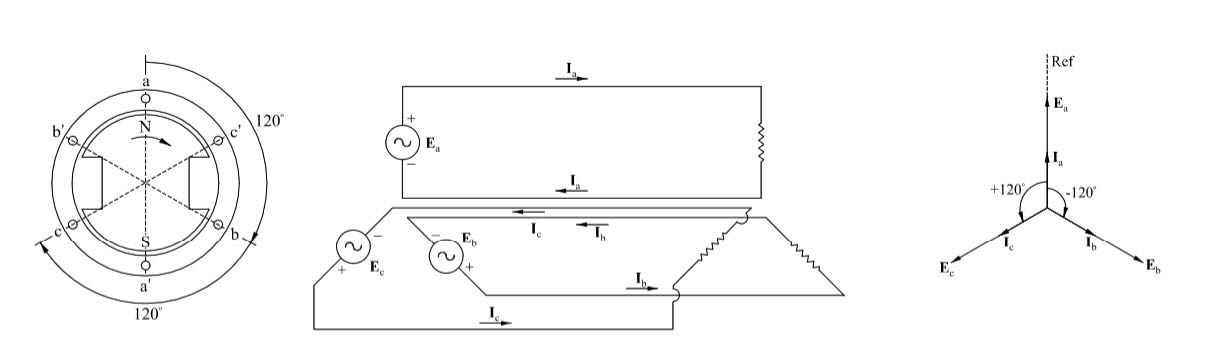
\includegraphics[scale=0.25]{3-phase-resistive.png}
	\end{center}
	\begin{align*}
		e_{a}&=E_{m}\cos(\omega t)\\
		i_{a}&=I_{m}\cos(\omega t)\\\\
		e_{b}&=E_{m}\cos(\omega t-120^{\circ})\\
		i_{b}&=I_{m}\cos(\omega t-120^{\circ})\\\\
		e_{c}&=E_{m}\cos(\omega t-240^{\circ})\\
		&=E_{m}\cos(\omega t+120^{\circ})\\
		i_{c}&=I_{m}\cos(\omega t-240^{\circ})\\
		&=I_{m}\cos(\omega t+120^{\circ})\\\\
		P_{Tot}&=P_{a}+P_{b}+P_{c}\\
		&=1.5E_{m}I_{m}\\
		&=3E_{RMS}I_{RMS}
	\end{align*}
	\subsection{3-Phase Connections:}
	\begin{center}
		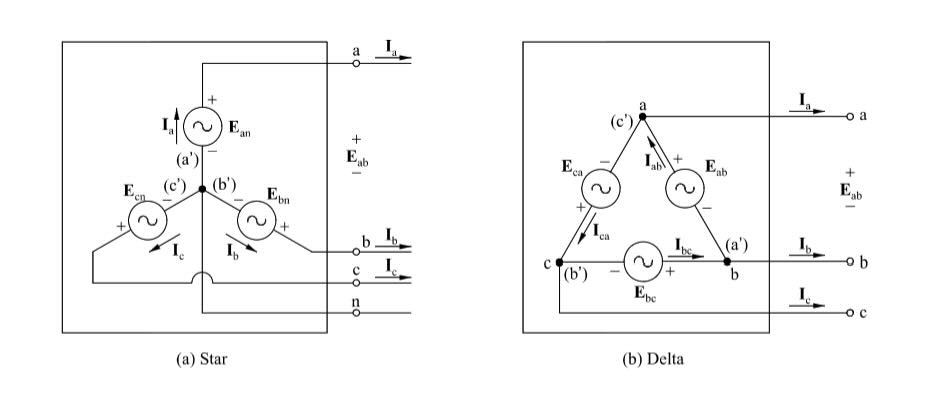
\includegraphics[scale=0.35]{3-phase-connections.png}
	\end{center}
	\subsection{Balanced Systems:}
	\begin{center}
		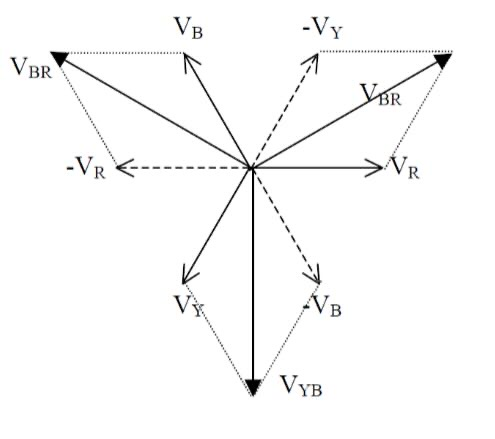
\includegraphics[scale=0.5]{3-phase-balanced.png}
	\end{center}
	\begin{itemize}
		\item Angles between phases is $120^{\circ}$
		\item Magnitudes are all equal
		\item $V_{L}$ would be $30^{\circ}$ leading nearest phase voltage
		\item $|V_{L}|$ is $\sqrt{3}|V_{P}|$
	\end{itemize}
	\begin{align*}
		I_{L}&=I_{P}\\
		|V_{L}|&=\sqrt{3}|V_{P}|\\
		|I_{L}|&=\sqrt{3}|I_{P}|
	\end{align*}
	\subsection{3-Phase Device Connection:}
	\begin{center}
		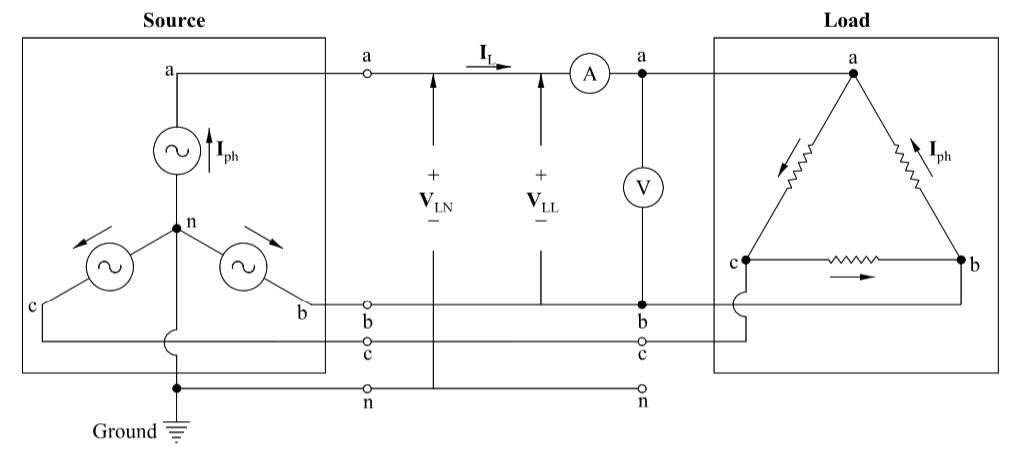
\includegraphics[scale=0.25]{load-connection.png}
	\end{center}
	The delta-star and star-delta conversions can be done. The only requirement is that the device voltage ratings must be compatitable.
	\subsection{Phase Sequence:}
	The phase sequence denotes which phase becomes succesively positive.
	\begin{center}
	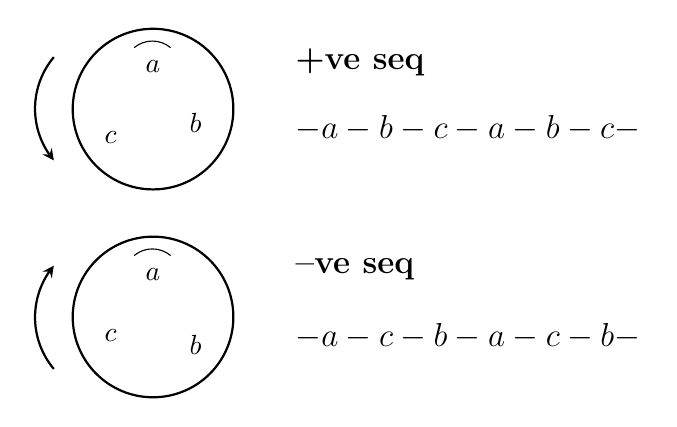
\begin{tikzpicture}[scale=1.2, line width=0.8pt]
	    % ================= TOP ROW: POSITIVE SEQUENCE =================
	    \begin{scope}[shift={(0, 2.2)}]
		% Main Circle
		\draw[thick] (0, 0) circle (0.85);

		% Labels inside Circle
		\node at (0, 0.45) {$a$};
		\draw[thin] (-0.2, 0.65) arc (130:50:0.3); % Arc over 'a'
		\node at (0.45, -0.15) {$b$};
		\node at (-0.45, -0.3) {$c$};

		% Counter-clockwise Rotation Arrow
		\draw[->, >=stealth, thick] (-1.05, 0.55) arc (140:220:0.85);

		% Text Description
		\node[right, font=\large] at (1.4, 0.5) {\textbf{+ve seq}};
		\node[right, font=\large] at (1.4, -0.2) {$-a-b-c-a-b-c-$};
	    \end{scope}

	    % ================= BOTTOM ROW: NEGATIVE SEQUENCE =================
	    \begin{scope}[shift={(0, 0)}]
		% Main Circle
		\draw[thick] (0, 0) circle (0.85);

		% Labels inside Circle
		\node at (0, 0.45) {$a$};
		\draw[thin] (-0.2, 0.65) arc (130:50:0.3); % Arc over 'a'
		\node at (0.45, -0.3) {$b$};
		\node at (-0.45, -0.2) {$c$};

		% Clockwise Rotation Arrow
		\draw[->, >=stealth, thick] (-1.05, -0.55) arc (220:140:0.85);

		% Text Description
		\node[right, font=\large] at (1.4, 0.5) {\textbf{--ve seq}};
		\node[right, font=\large] at (1.4, -0.2) {$-a-c-b-a-c-b-$};
	    \end{scope}

	\end{tikzpicture}
	\end{center}
	\subsection{3-Phase Solutions:}
	\begin{itemize}
		\item Most 3-Phase system can be though of as balanced
		\item To solve an unbalanced 3-phase system is quite complex
	\end{itemize}
	\subsection{Symmetrical Component Analysis:}
	Any unbalanced system can be split up into a series of balanced systems.
	\begin{itemize}
		\item Same phase sequence (Positive)
		\item Opposite phase sequence (Negative)
		\item In phase quantities (Zero)
	\end{itemize}
	\subsection{Unbalanced Decomposition:}
	\begin{center}
		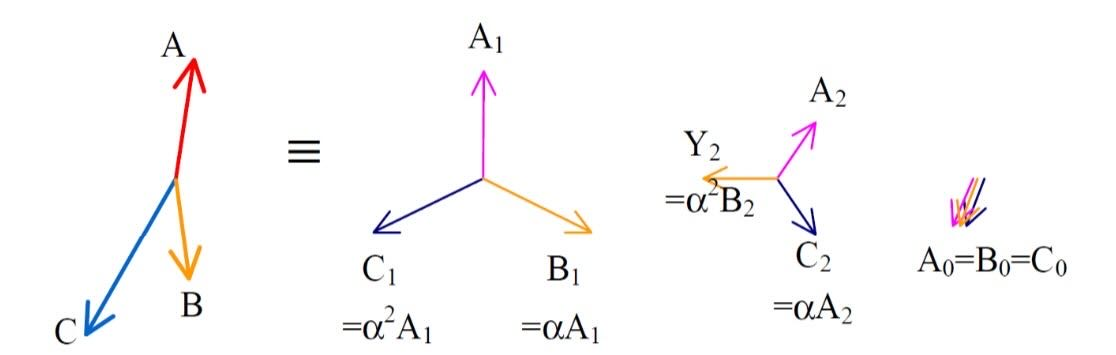
\includegraphics[scale=0.25]{unbalanced-decomp.png}
	\end{center}
	$$\alpha=1\angle120^{\circ}$$
	\begin{align*}
		A&=A_{0}+A_{1}+A_{2}=A_{0}+A_{1}+A_{2}\\
		B&=B_{0}+B_{1}+B_{2}=A_{0}+\alpha^{2}A_{1}+\alpha A_{2}\\
		C&=C_{0}+C_{1}+C_{2}=A_{0}+\alpha A_{1}+\alpha^{2}A_{2}\\\\
		&\begin{bmatrix}
			1 & 1 & 1\\
			1 & \alpha^{2} & \alpha\\
			1 & \alpha & \alpha^{2}
		\end{bmatrix}
		\begin{bmatrix}
			A_{0}\\
			A_{1}\\
			A_{2}
		\end{bmatrix}
	\end{align*}
	\subsection{Balanced Analysis:}
	\begin{center}
		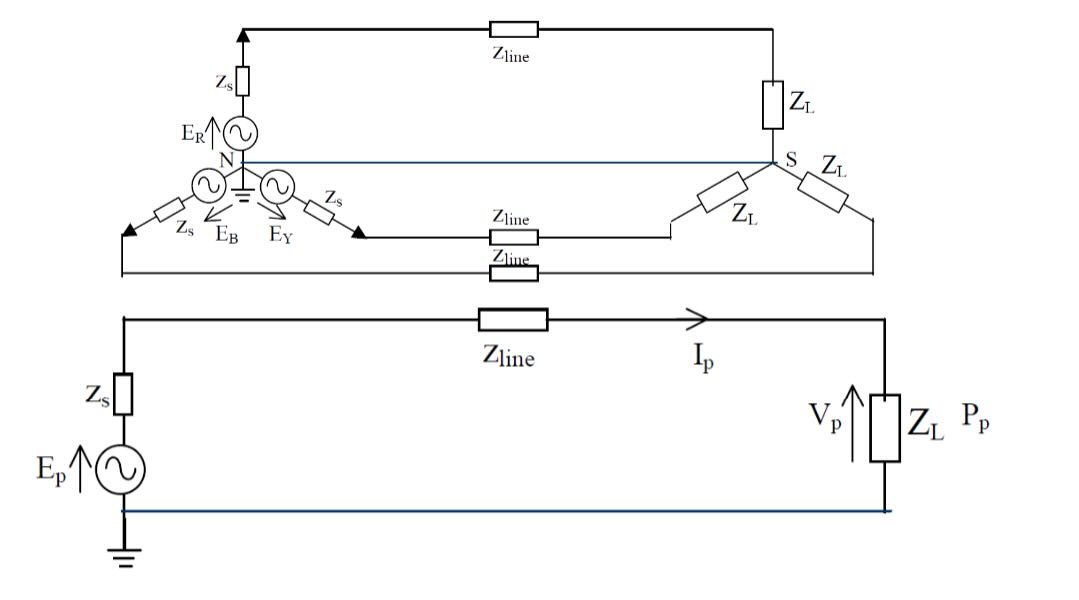
\includegraphics[scale=0.25]{balanced-analysis.png}
	\end{center}
	\subsubsection{Wye Connection}
	$$I_{P}=I_{L}$$
	$$V_{P}=\frac{V_{L}}{\sqrt{3}}$$
	\subsubsection{Delta Connection}
	$$V_{P}=V_{L}$$
	$$I_{P}=\frac{I_{L}}{\sqrt{3}}$$
	\subsubsection{All}
	$$S_{3P}=3V_{P}I_{P}=\sqrt{3}V_{L}I_{L}$$
	$$P_{1P}=\frac{P_{3P}}{3}$$
	\subsection{Selecting Number of Phases:}
	The number of phases for a power system is determined by transmission system economies. That is done by analyzing the amount of power transferred per conductor. With the assumption that the size of the return conductor is equal to that phase conductor.
	\begin{center}
	\begin{tabular}{ c | c c c }
		System & Power Rating & No. Conductors & Power per Conductor\\
		\hline\\
		1-Phase & P & 2 & 0.5P\\
		2-Phase & 2P & 3 & 0.667P\\
		3-Phase & 3P & 4 & 0.75P\\
		4-Phase & 4P & 5 & 0.8P
	\end{tabular}
	\end{center}

\end{document}
